\documentclass[10pt]{article}
\usepackage[margin=1in]{geometry} 

\usepackage{amsmath,amsthm,amssymb,graphicx,amsfonts}

\usepackage{float}
\usepackage{caption,subcaption} % para las figuras
\usepackage{wrapfig}

\usepackage{comment}

\usepackage[utf8]{inputenc} %tildes
\usepackage[spanish]{babel}

\usepackage{enumerate}

\usepackage{color}   %May be necessary if you want to color links
\usepackage{hyperref}
\hypersetup{
	colorlinks=true, %set true if you want colored links
	linktoc=all,     %set to all if you want both sections and subsections linked
	linkcolor=blue,  %choose some color if you want links to stand out
}

\begin{document}
	
\title{Población Penitenciaria en Argentina\\ 2002 a 2017 \\
	\begin{small}
		Tutor: Franco Camporeale
	\end{small}}
\author{\small{Nahuel Almeida, María Lucía Pappaterra, Javier ¿?}}

\maketitle

\section{Análisis estadístico de variables}

Seleccionar un conjunto de al menos cuatro variables que resulten de interés.

\begin{enumerate}
	\item Usar distintos tipos de gráficos para describir sus distribuciones
	\item Analizar Outliers
	\item Calcular estadísticos clásicos (media, mediana, moda, desviación estandar)
\end{enumerate}

Las variables elegidas fueron: edad, duración de condena, diferencia entre fecha de condena y fecha de detención, cantidad de delitos por interno.

\subsection{Edad}

En la figura \ref{fig:edad} mostramos la distribuci\'on de edades de los internos, junto con su suma acumulada. Podemos ver que la mayor\'ia de los internos son personas j\'ovenes, y que el n\'umero de internos decae fuertemente con la edad. En el histograma se observa que hay registros de personas con edad cercana a 0 años. En realidad, se trata de 369 registros con edad igual a 0 años. Estos casos podr\'ian tratarse de un error de carga, o podr\'ian correspondan a ni\~nos nacidos dentro de los establecimientos. Observando en detalle esos registros, se puede ver que la segunda opci\'on es improbable, dado que esos registros tienen informaci\'on en otros campos que corresponden a internos que han cometido delitos.  Los dem\'as registros que podr\'ian ser considerados como outliers son los correspondientes a menores de edad. En este caso, existen 8 registros de personas de 16 a\~nos y 11 registros de personas de 17 a\~nos. Como esta cantidad es baja y no afecta la estad\'istica, decidimos incluirlos en el an\'alisis.

\begin{figure}[H]
	\centering
	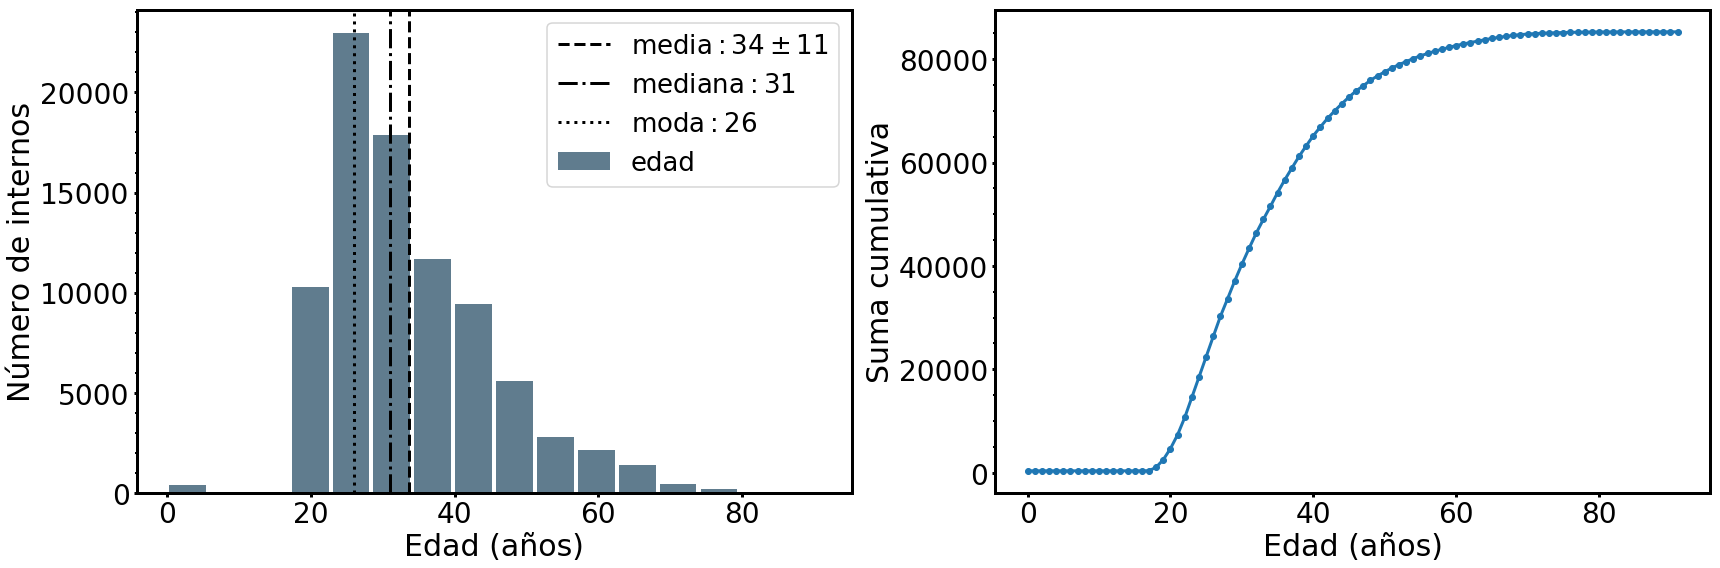
\includegraphics[scale=0.28]{graficos/edad.png}
	\caption{Histograma de edades de los internos, junto con su la suma acumulada. \label{fig:edad}}
\end{figure}

\subsection{Duración de condena}

En la figura \ref{fig:duracion_condena} mostramos el histograma de duraci\'on de condenas, junto con su suma cumulativa complemantaria. 

\begin{figure}[H]
	\centering
	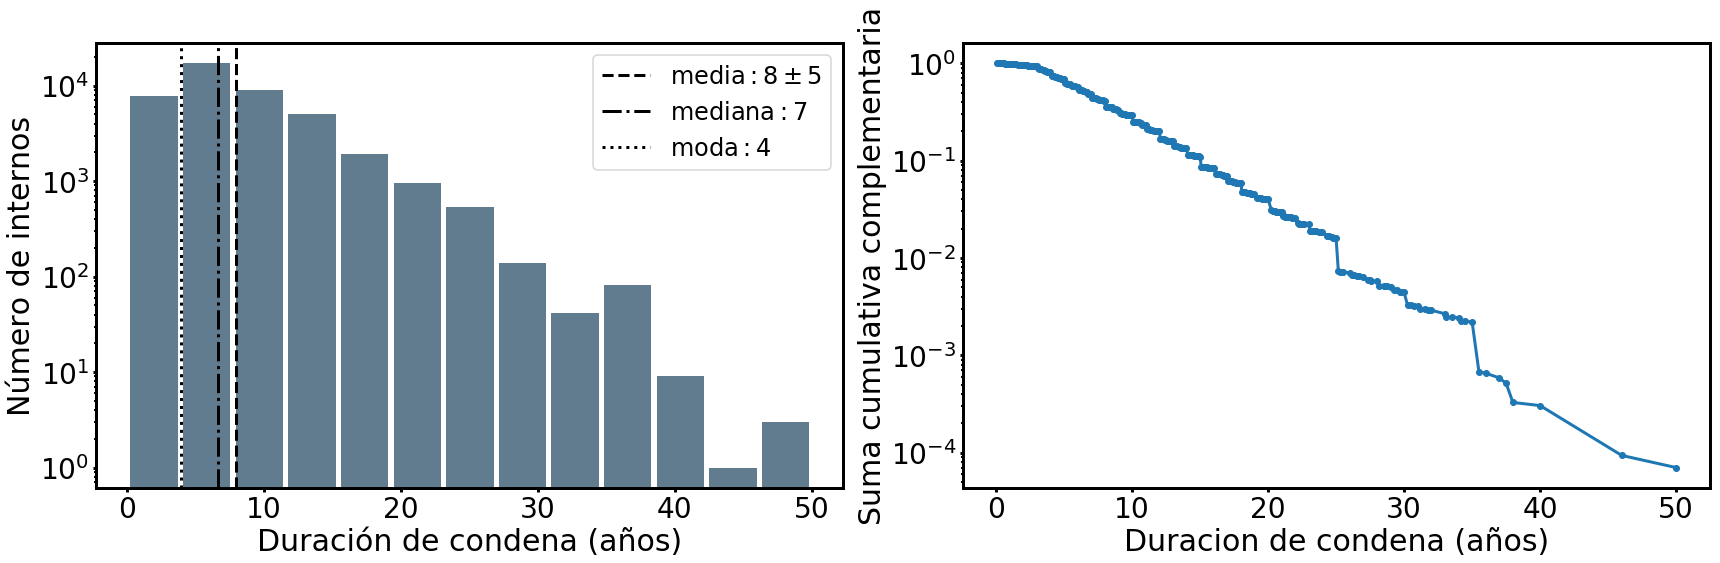
\includegraphics[scale=0.28]{graficos/duracion_condena.png}
	\caption{Histograma de la duraci\'on de condenas y su suma cumulativa complementaria. \label{fig:duracion_condena}}
\end{figure}

\subsection{variable3}

\begin{figure}[H]
	\centering
	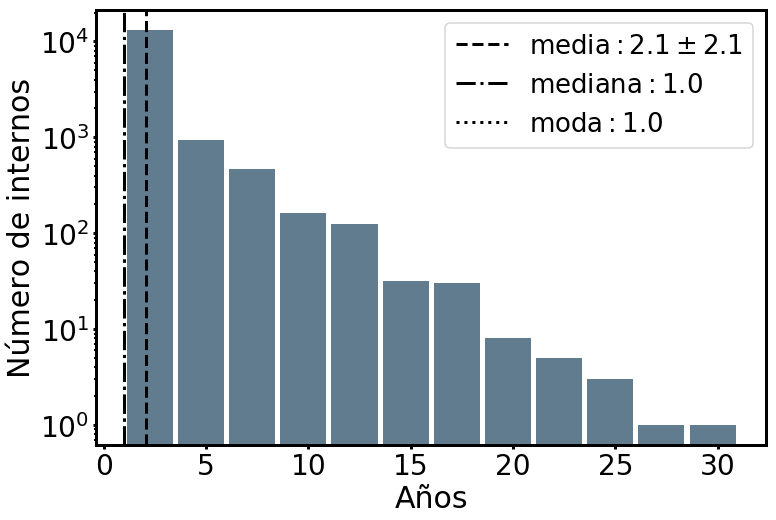
\includegraphics[scale=0.3]{graficos/diff_condenado_detencion.png}
	\caption{Histograma de los tiempos transcurridos entre la fecha de detenci\'on y la fecha de condena. \label{fig:tiempo_detencion_condena}}
\end{figure}

\subsection{Cantidad de delitos por interno}

\begin{figure}[H]
	\centering
	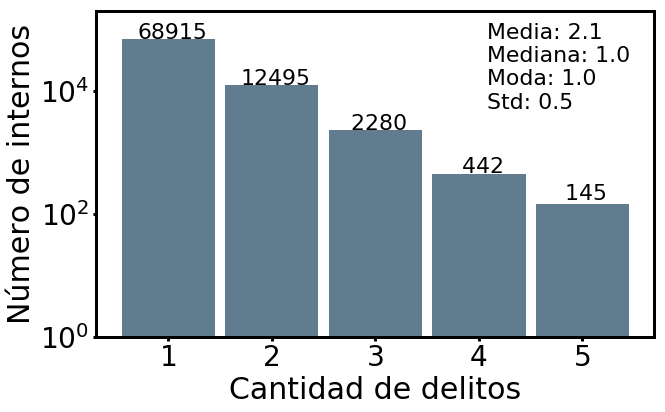
\includegraphics[scale=0.4]{graficos/cantidad_delitos.png}
	\caption{Histograma de la cantidad de delitos cometidos por cada interno. \label{fig:cantidad_delitos}}
\end{figure}

\section{Evolución de variables en el tiempo}
Seleccionar dos variables y graficar cómo fueron cambiando desde 2002 a 2017. Para ello se tiene que utilizar el siguiente conjunto de datos: \url{https://github.com/camporeale/Datos/raw/master/sneep_2002_2017_diplodatos.zip}\\

Las variables elegidas fueron situación legal y participación en programas educativos.

\subsection{Situación legal}

Veamos cómo evoluciona la cantidad de internos condenados y procesados a lo largo de los años, y si nuestro análisis se condice con el de la nota de chequeado: \url{https://chequeado.com/ultimas-noticias/martin-casares-por-primera-vez-en-la-historia-en-2017-el-porcentaje-de-condenados-supero-al-de-procesados/}

\begin{figure}[H]
	\centering
	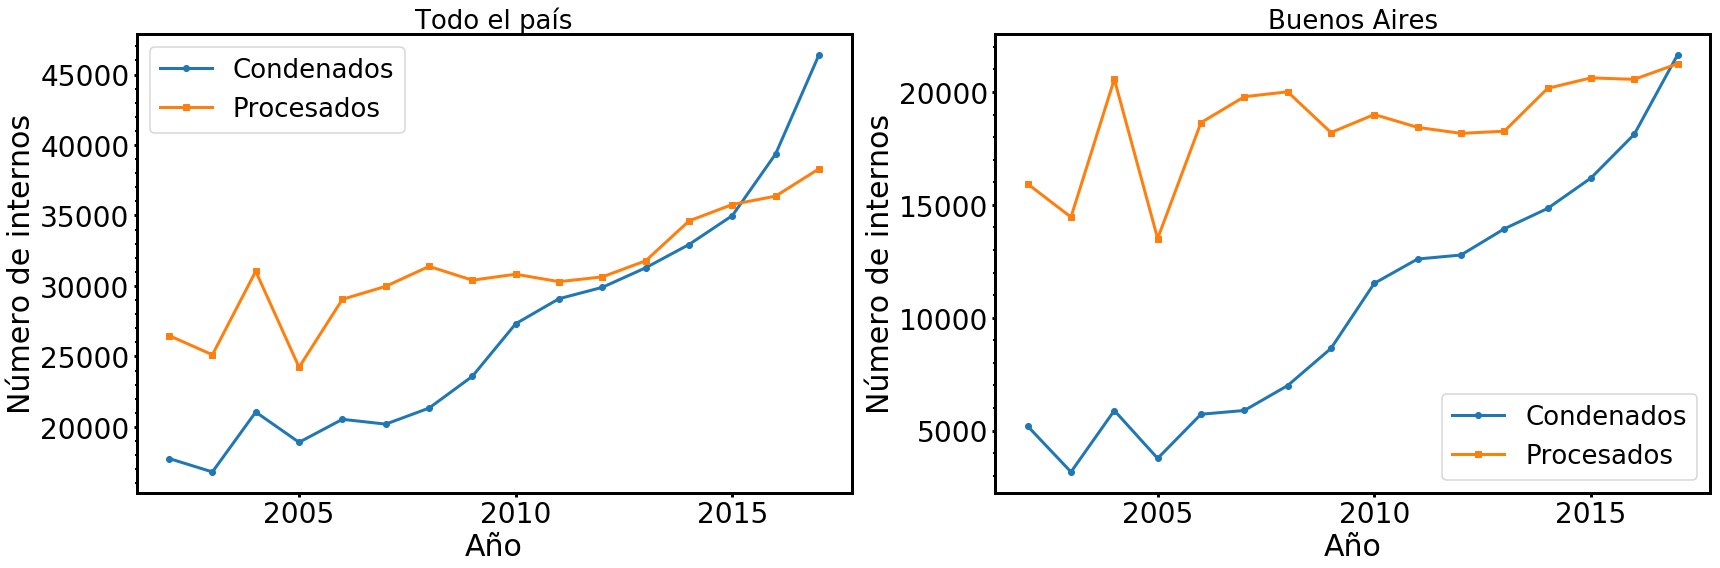
\includegraphics[scale=0.28]{graficos/situacion.png}
	\caption{}
\end{figure}

\begin{figure}[H]
	\centering
	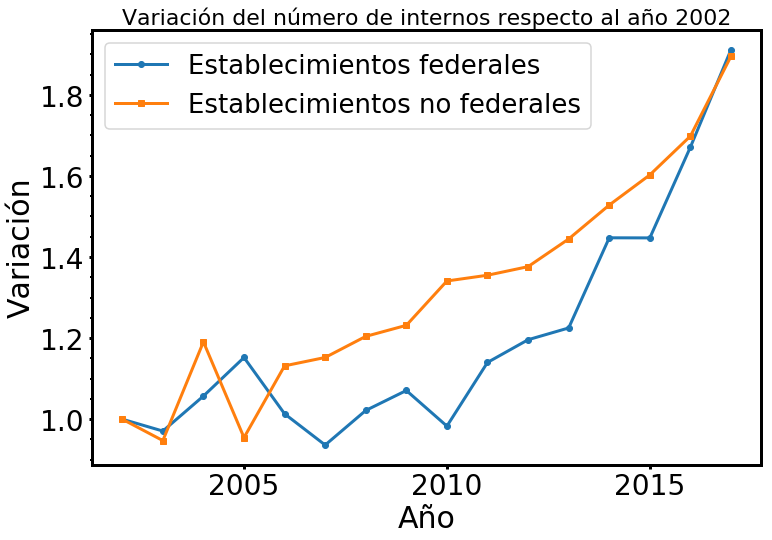
\includegraphics[scale=0.3]{graficos/variacion.png}
	\caption{}
\end{figure}

\subsection{Participación en programas educativos}

Queremos ver cómo varía la proporción de internos que participa en programas educativos a lo largo del tiempo.

\begin{figure}[H]
	\centering
	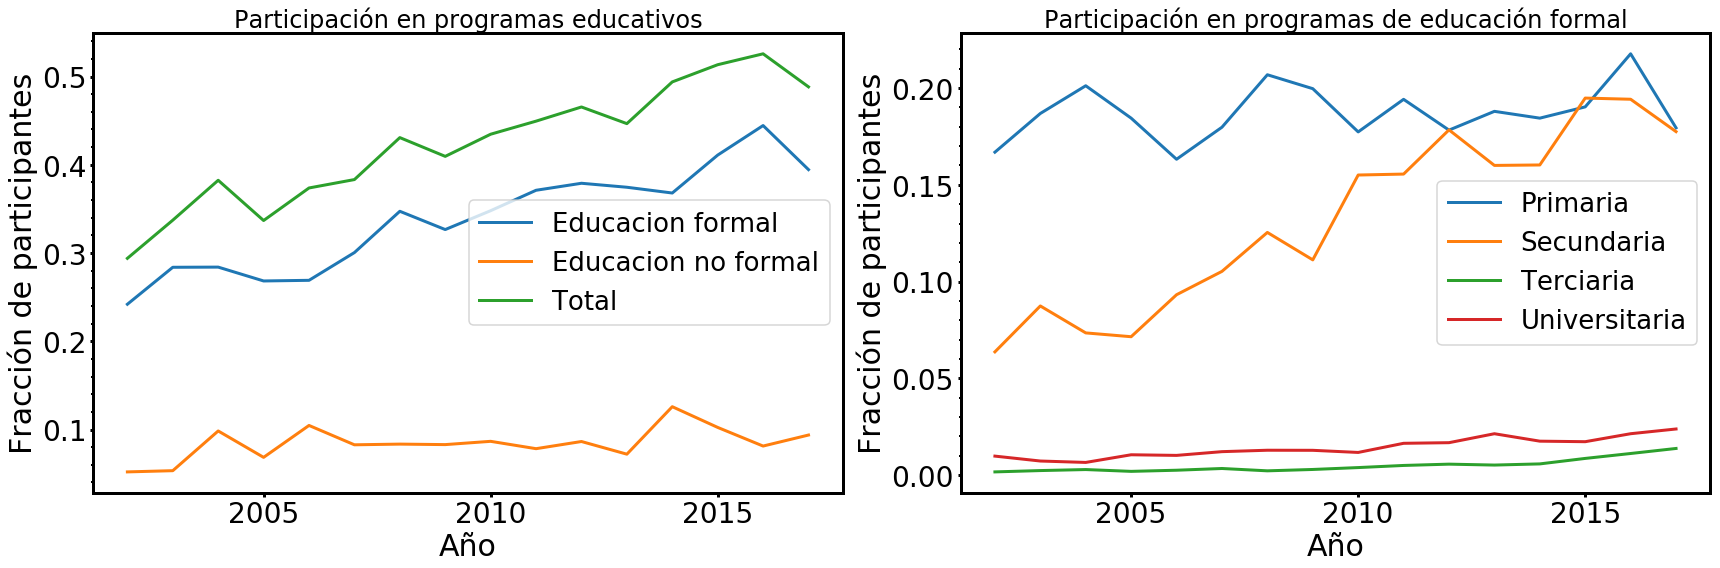
\includegraphics[scale=0.28]{graficos/educacion.png}
	\caption{}
\end{figure}

\section{Análisis de probabilidades condicionales}
Tomar al menos dos pares de variables y realizar un análisis del tipo:

\begin{itemize}
	\item ¿Cuál es el porcentaje de internos argentinos y extranjeros? ¿Cómo varían esos números de acuerdo a si el establecimiento es federal o no federal?
	\item ¿Cuál es la probabilidad de que el interno haya sido lesionado en el último año dado que está en una prisión en Buenos Aires? ¿Y en Córdoba?
	\item ¿Cuál es la probabilidad de que se le otorguen salidas provisorias dado que esté casado/a? ¿Y siendo soltero?
\end{itemize}

\begin{figure}[H]
	\centering
	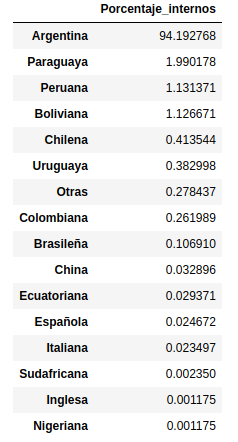
\includegraphics[scale=0.6]{graficos/nacionalidad.png}
	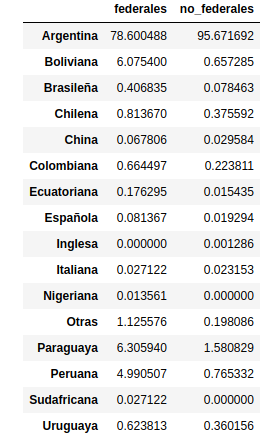
\includegraphics[scale=0.6]{graficos/nacionalidad_tipo_establecimiento.png}
	\caption{}
\end{figure}




\end{document}